%=============================================================================
% 模块二:图像数学/物理基础
%=============================================================================

\section{图像的数字表示}

\begin{frame}[fragile]{图像的底层本质:矩阵 (Matrix)}
	\begin{columns}
		\column{0.5\textwidth}
		\begin{itemize}
			\item 一张灰度图 = 一个 \textbf{二维矩阵}。
			\item 矩阵中的每个元素称为 \highlight{像素 (Pixel)}。
			\item 常用数据类型:\texttt{uint8} (0-255)。
		\end{itemize}
		\column{0.5\textwidth}
		\begin{center}
			\small
			$\begin{bmatrix}
					255 & 255 & 254 \\
					120 & 0   & 118 \\
					255 & 253 & 255
				\end{bmatrix}$
			\vspace{0.2cm}
			\\ (矩阵数值 $\to$ 图像亮度)
		\end{center}
	\end{columns}
	\begin{alertblock}{注意坐标系!}
		计算机图像坐标系:\textbf{左上角为原点 (0,0)},X轴向右,Y轴向 \highlight{下}。
	\end{alertblock}
\end{frame}

\begin{frame}[fragile]{彩色图像:RGB 三通道}
	\begin{itemize}
		\item 彩色图像 = 三个二维矩阵堆叠 (\textbf{三维张量})。
		\item 每个通道代表一种颜色光的强度。
	\end{itemize}
	\begin{center}
		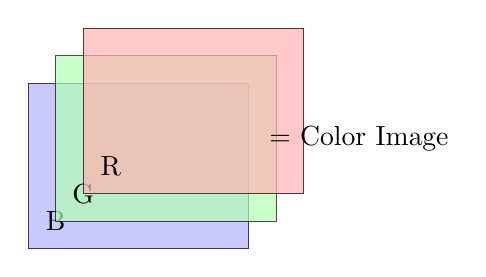
\begin{tikzpicture}[scale=0.7]
			\draw[fill=blue!30, opacity=0.7] (0,0) rectangle (4,3); \node at (0.5, 0.5) {B};
			\draw[fill=green!30, opacity=0.7] (0.5,0.5) rectangle (4.5,3.5); \node at (1, 1) {G};
			\draw[fill=red!30, opacity=0.7] (1,1) rectangle (5,4); \node at (1.5, 1.5) {R};
			\node at (6, 2) {= Color Image};
		\end{tikzpicture}
	\end{center}
	\textbf{OpenCV 的特殊性:} 默认读取顺序是 \highlight{BGR},而非 RGB。
\end{frame}

\begin{frame}[fragile]{互动练习:调色盘}
	如果一个像素的 RGB 值为以下数值,它是什么颜色?
	\begin{table}
		\centering
		\begin{tabular}{cccc}
			\toprule
			R   & G   & B   & 预测颜色                                  \\
			\midrule
			255 & 255 & 0   & \uncover<2->{\textcolor{yellow}{黄色}}  \\
			0   & 255 & 255 & \uncover<3->{\textcolor{cyan}{青色/浅蓝}} \\
			128 & 128 & 128 & \uncover<4->{\textcolor{gray}{灰色}}    \\
			0   & 0   & 0   & \uncover<5->{\textbf{黑色}}             \\
			\bottomrule
		\end{tabular}
	\end{table}
\end{frame}

\begin{frame}[fragile]{像素级操作:NumPy数组操作}
	\begin{columns}
		\column{0.5\textwidth}
		\textbf{基础索引与切片:}
		\begin{lstlisting}[language=Python, basicstyle=\ttfamily\tiny]
# 获取单个像素
pixel = img[100, 200]  # 返回[B, G, R]

# 获取红色通道
red_channel = img[:, :, 2]

# 获取左上角100x100区域
top_left = img[0:100, 0:100]

# 水平翻转(左右颠倒)
flipped = img[:, ::-1, :]
		\end{lstlisting}

		\vspace{0.2cm}
		\textbf{条件操作:}
		\begin{lstlisting}[language=Python, basicstyle=\ttfamily\tiny]
# 找出所有暗像素(值 < 128)
dark_pixels = img < 128

# 将暗像素增强
img[dark_pixels] = img[dark_pixels] * 1.2
		\end{lstlisting}

		\column{0.5\textwidth}
		\textbf{统计操作:}
		\begin{lstlisting}[language=Python, basicstyle=\ttfamily\tiny]
# 计算平均值
mean_val = np.mean(img)

# 计算标准差
std_val = np.std(img)

# 找最大最小值
max_val = np.max(img)
min_val = np.min(img)

# 计算非零像素数量
nonzero_count = np.count_nonzero(img)
		\end{lstlisting}

		\vspace{0.2cm}
		\begin{alertblock}{重要提示}
		NumPy切片是\textbf{视图(view)}而非副本,修改切片会影响原图!
		如果需要独立副本,使用\texttt{img.copy()}
		\end{alertblock}
	\end{columns}
\end{frame}

\begin{frame}[fragile]{像素级操作:手动实现灰度化}
	\textbf{原理:} $Gray = R \times 0.299 + G \times 0.587 + B \times 0.114$

	\begin{columns}
		\column{0.5\textwidth}
		\textbf{方法1:手动循环(学习用,不推荐)}
		\begin{lstlisting}[language=Python, basicstyle=\ttfamily\tiny]
def manual_grayscale(img):
    """手动实现灰度化"""
    h, w, c = img.shape
    gray = np.zeros((h, w), dtype=np.uint8)

    for i in range(h):
        for j in range(w):
            b, g, r = img[i, j]
            gray[i, j] = int(0.299*r +
                             0.587*g +
                             0.114*b)
    return gray
		\end{lstlisting}
		\textit{缺点:速度慢,不推荐生产环境使用}

		\column{0.5\textwidth}
		\textbf{方法2:向量化操作(推荐)}
		\begin{lstlisting}[language=Python, basicstyle=\ttfamily\tiny]
def grayscale_vectorized(img):
    """向量化实现灰度化"""
    # 方法1:矩阵运算
    b, g, r = cv2.split(img)
    gray = 0.299*r + 0.587*g + 0.114*b
    return gray.astype(np.uint8)

    # 方法2:点积(更简洁)
    weights = np.array([0.114, 0.587, 0.299])
    gray = img.dot(weights).astype(np.uint8)
    return gray
		\end{lstlisting}
		\textit{优点:速度快,利用NumPy向量化加速}
	\end{columns}

	\vspace{0.3cm}
	\begin{center}
		\textbf{性能对比:} 手动循环 \texttt{200ms} vs 向量化操作 \texttt{5ms}(快40倍)
	\end{center}
\end{frame}

\begin{frame}[fragile]{像素级操作:亮度调整的"溢出"陷阱}
	\begin{columns}
		\column{0.5\textwidth}
		\textbf{❌ 错误做法:}
		\begin{lstlisting}[language=Python, basicstyle=\ttfamily\tiny]
img = cv2.imread('exam.jpg')

# 直接相加
bright = img + 50

# 问题:如果像素值是220,
# 220 + 50 = 270
# 但uint8的范围是0-255
# 270会截断为14(或绕回)
# 导致图像出现噪点!
		\end{lstlisting}

		\vspace{0.2cm}
		\begin{alertblock}{为什么?}
		uint8类型:8位无符号整数\\
		范围:$[0, 255]$\\
		溢出:截断到边界值
		\end{alertblock}

		\column{0.5\textwidth}
		\textbf{✅ 正确做法:}
		\begin{lstlisting}[language=Python, basicstyle=\ttfamily\tiny]
# 方法1:使用np.clip
bright = np.clip(
    img.astype(np.int32) + 50,
    0, 255
).astype(np.uint8)

# 方法2:使用cv2.add(推荐)
bright = cv2.add(
    img,
    np.array([50.0])
)

# 方法3:使用convertScaleAbs
bright = cv2.convertScaleAbs(
    img,
    alpha=1.0,  # 对比度
    beta=50     # 亮度增量
)
		\end{lstlisting}
	\end{columns}

	\vspace{0.3cm}
	\begin{block}{核心原理}
		先转为int32类型(支持大范围),再clip到[0, 255],最后转回uint8
	\end{block}
\end{frame}

% 直方图理论
\begin{frame}[fragile]{图像的统计特性:直方图 (Histogram)}
	\begin{columns}
		\column{0.5\textwidth}
		\textbf{什么是直方图?}
		\begin{itemize}
			\item 横坐标:亮度级别 (0-255)
			\item 纵坐标:该亮度像素出现的频次
		\end{itemize}

		\textbf{在阅卷中的意义:}
		\begin{itemize}
			\item \highlight{曝光检查}:判断照片是否太暗或过曝
			\item \highlight{二值化参考}:寻找波谷作为分割阈值
		\end{itemize}

		\column{0.5\textwidth}
		\begin{lstlisting}[language=Python, basicstyle=\ttfamily\tiny]
import cv2
import matplotlib.pyplot as plt

# 计算直方图
img = cv2.imread('exam.jpg',
                 cv2.IMREAD_GRAYSCALE)
hist = cv2.calcHist([img], [0], None,
                    [256], [0, 256])

plt.plot(hist)
plt.title('Pixel Intensity Distribution')
plt.show()
		\end{lstlisting}

		\begin{center}
			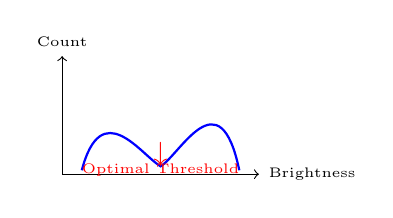
\begin{tikzpicture}[scale=0.5]
				\draw[->] (0,0) -- (5,0) node[right] {\tiny Brightness};
				\draw[->] (0,0) -- (0,3) node[above] {\tiny Count};
				\draw[thick, blue] (0.5,0.1) .. controls (1,2) and (2,0.5) .. (2.5,0.2) .. controls (3,0.5) and (4,2.5) .. (4.5,0.1);
				\node[red] at (2.5, 0.5) {$\downarrow$};
				\node[red, below] at (2.5, 0.5) {\tiny Optimal Threshold};
			\end{tikzpicture}
		\end{center}
	\end{columns}
\end{frame}

\begin{frame}[fragile]{直方图形态分析:试卷照片的曝光诊断}
	\textbf{场景:}自动判断试卷照片的质量

	\begin{columns}
		\column{0.5\textwidth}
		\textbf{1. 正常曝光(双峰分布)}
		\begin{itemize}
			\item 白纸(高亮度)+ 黑字(低亮度)
			\item 波谷在中间,适合二值化
			\item \textcolor{green!60!black}{\textbf{阅卷理想状态}}
		\end{itemize}

		\textbf{2. 欠曝(左偏分布)}
		\begin{itemize}
			\item 大部分像素集中在暗部
			\item 可能是光照不足
			\item 需要亮度增强
		\end{itemize}

		\textbf{3. 过曝(右偏分布)}
		\begin{itemize}
			\item 大部分像素集中在亮部
			\item 可能是闪光灯太强
			\item 需要降低亮度
		\end{itemize}

		\column{0.5\textwidth}
		\begin{lstlisting}[language=Python, basicstyle=\ttfamily\tiny]
def check_exposure(img):
    """检查图像曝光情况"""
    gray = cv2.cvtColor(img,
                       cv2.COLOR_BGR2GRAY)

    # 计算平均亮度
    mean_brightness = np.mean(gray)

    # 判断曝光状态
    if mean_brightness < 80:
        return "欠曝,建议增强"
    elif mean_brightness > 200:
        return "过曝,建议降低"
    else:
        return "曝光正常"

# 使用
status = check_exposure(img)
print(f"曝光状态: {status}")
		\end{lstlisting}
	\end{columns}
\end{frame}

\begin{frame}[fragile]{图像缩放:插值算法对比}
	\textbf{问题:}cv2.resize 时,像素是如何"凭空产生"或"消失"的?

	\begin{columns}
		\column{0.5\textwidth}
		\begin{lstlisting}[language=Python, basicstyle=\ttfamily\tiny]
import cv2
import numpy as np

img = cv2.imread('exam.jpg')
h, w = img.shape[:2]

# 1. 最近邻插值(最快)
# 取最近的像素值,会有马赛克
near = cv2.resize(img, (w*2, h*2),
                  interpolation=cv2.INTER_NEAREST)

# 2. 双线性插值(默认)
# 周围4个像素加权平均,较平滑
linear = cv2.resize(img, (w*2, h*2),
                   interpolation=cv2.INTER_LINEAR)

# 3. 双三次插值(最慢但最好)
# 周围16个像素加权平均
cubic = cv2.resize(img, (w*2, h*2),
                  interpolation=cv2.INTER_CUBIC)
		\end{lstlisting}

		\column{0.5\textwidth}
		\textbf{插值效果对比:}
		\begin{itemize}
			\item \textbf{最近邻}:
			      \begin{itemize}
				      \item 速度:最快
				      \item 质量:有锯齿
				      \item 应用:像素风游戏
			      \end{itemize}
			\item \textbf{双线性}:
			      \begin{itemize}
				      \item 速度:中等
				      \item 质量:较平滑
				      \item 应用:日常缩放
			      \end{itemize}
			\item \textbf{双三次}:
			      \begin{itemize}
				      \item 速度:最慢
				      \item 质量:最平滑
				      \item 应用:高质量缩放
			      \end{itemize}
		\end{itemize}

		\vspace{0.2cm}
		\textbf{阅卷建议:}
		\begin{itemize}
			\item 缩小用 \texttt{INTER\_AREA}(抗锯齿)
			\item 放大用 \texttt{INTER\_CUBIC}(高质量)
		\end{itemize}
	\end{columns}
\end{frame}
